\begin{figure}[b]
    \centering
    \begin{tabular}{@{}c@{}c@{}c@{}}
        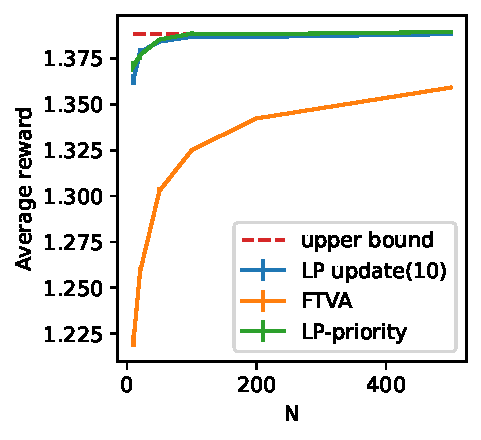
\includegraphics[width=0.33\linewidth]{random-example3_functionN}
        &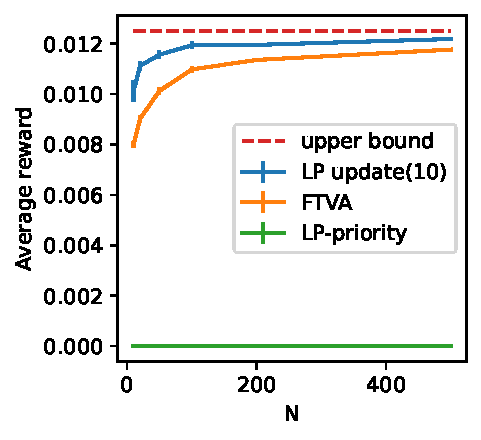
\includegraphics[width=0.33\linewidth]{counter-example-Hong_functionN.pdf}
        &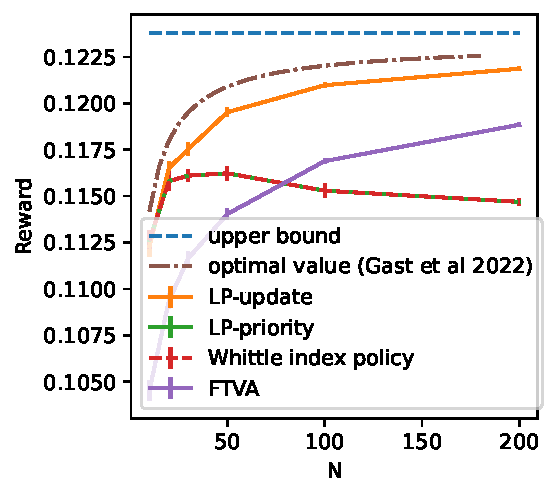
\includegraphics[width=0.33\linewidth]{counter-example-GGY2_perfN.pdf}\\
        (a) Random example
        &(b) Example \cite{HXCW23}
        &(c) Example \cite{chen:tel-04068056}
    \end{tabular}
    \caption{Performance as a function of $N$}
    \label{fig:perf_function_of_N}
\end{figure}

\section{Numerical illustrations}
\label{sec:numerical}

We illustrate numerically the performance of the LP-update policy, showing that it performs very well in practice and outperforms classical heuristics in most cases. We choose to compare against two heuristics of the literature: the LP-priority policy of \cite{GGY23} and the follow the virtual advice policy (FTVA) of \cite{HXCW23}. The LP-priority policy computes a solution to \eqref{EQ::VOPTDYN-Tinf} and uses it to compute a priority order on states, arms are then pulled according to this priority order.  The LP-priority policy is an index policy ---similarly to Whittle index policy--- but has the advantage of being always defined, whereas Whittle index policy is only defined under a technical condition known as indexability. The LP-update policy has only been shown to be optimal under the UGAP assumption. %till the budget is exhausted.
FTVA constructs a virtual collection of $N$ arms which follow the solution to \eqref{EQ::VOPTDYN-Tinf}. When a virtual arm is pulled, the corresponding real arm is pulled if the budget allows it, otherwise the real arm is left alone. If the virtual and real arm choose the same actions, they evolve identically, otherwise independently. We choose these two heuristics because they are natural and simple to implement and do not rely on hard-to-tune hyperparameters (further discussion for our choice can be found in the supplementary material along with choices for the parameters, see Appendix ~\ref{apx:parameters}).
%Appendix ~\ref{apx:parameters}). %All parameters are provided in Appendix~\ref{apx:parameters}.
We provide the parameters in Appendix~\ref{apx:parameters}.All codes are provided in supplementary material.
%In the future, a Github link will be provided.

\paragraph{Comparison on representative examples} For our first comparison, we consider three representative examples: a randomly generated example (in dimension 8), the main example used in \cite{HXCW23} and described in their Appendix~G.2 (abbreviated Example~\cite{HXCW23} in the following), and Example~2 of Figure~7.4 of \cite{chen:tel-04068056} (abbreviated Example~\cite{chen:tel-04068056}). We report the result in Figure~\ref{fig:perf_function_of_N}. We observe that in all three cases, both the LP-update and the FTVA policies are asymptotically optimal, but the LP-update policy outperforms FTVA substantially. The situation for LP-priority is quite different: as shown in \cite{GGY23}, in dimension 8, the LP-priority policy is asymptotically optimal for most of the randomly generated examples. This is the case for example (a) of Figure~\ref{fig:perf_function_of_N} for which LP-update and LP-priority give an essentially equivalent performance and are essentially almost optimal. The authors of \cite{chen:tel-04068056} provide the numerical value of the optimal policy for Example~\cite{chen:tel-04068056}, which can be done because $|\sspace|=3$. %We observe that 
The LP-update is very close to this value.


\paragraph{System dynamics:} To explore the difference of performance between the LP-update policy and FTVA, we study the dynamics of the different policies for the first two examples of Figure~\ref{fig:perf_function_of_N}. %We plot in 
Figure~\ref{fig:as_function_of_time} %the evolution of the system as a function of time
plots the evolution of the system over time (for a single trajectory). We observe that if the distance between $X_t$ and $x^*$ are similar for LP-update and FTVA, the rotated cost is much smaller for LP-update, which explains its good performance. 
\begin{figure}[ht]
    \centering
    \begin{tabular}{@{}c@{}c@{}@{}c@{}c}
        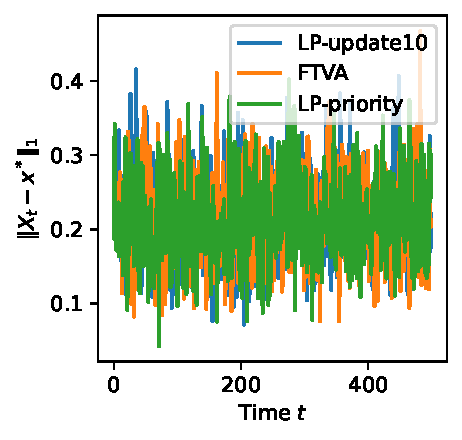
\includegraphics[width=0.25\linewidth]{random-example3-distance_N100.pdf}
        &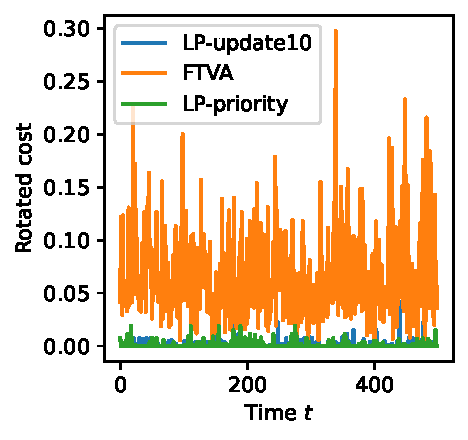
\includegraphics[width=0.25\linewidth]{random-example3-rotated-cost_N100.pdf}
        &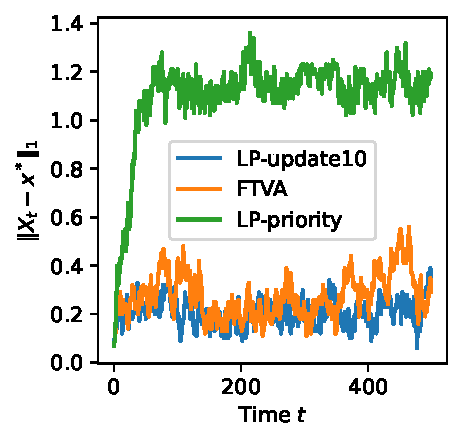
\includegraphics[width=0.25\linewidth]{counter-example-Hong-distance_N100.pdf}
        &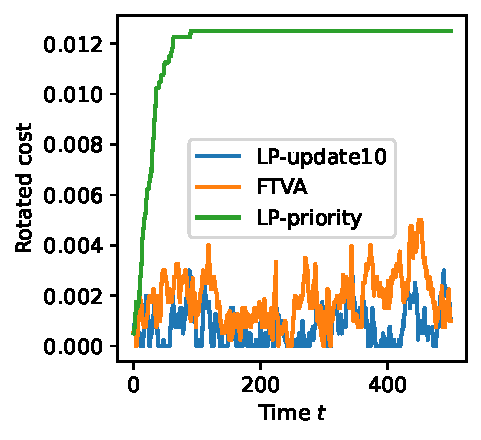
\includegraphics[width=0.25\linewidth]{counter-example-Hong-rotated-cost_N100.pdf}
        \\
        % Distance $\| X_t-x^*\|_1$
        % &Rotated cost
        % &Distance $\| X_t-x^*\|_1$
        % &Rotated cost\\
        \multicolumn{2}{c}{(a) Random example}
        &\multicolumn{2}{c}{(b) Example from Hong et al.}
    \end{tabular}

    \caption{Distance $\|X_t-x^*\|$ and rotated cost as a function of time for $N=100$.}
    \label{fig:as_function_of_time}
\end{figure}
To explore the system dynamics in more details, we focus on Example~\cite{chen:tel-04068056} and study the behavior of the LP-update, FTVA and LP-priority policy. In Figures~\ref{fig:example-chen}(a,b,c), we present a trajectory of each of the three policies: each orange point corresponds to a value of $X_t\in\Delta_\sspace$ (as this example is in dimension $|\sspace|=3$, the simplex $\Delta_\sspace$ can be represented as a triangle). This example has an unstable fixed point (Assumption~\ref{AS::stable} is not satisfied). Both LP-update and FTVA concentrate their behavior around this fixed point but the LP-priority policy exhibits two modes. %When concentrating on
The rotated cost (Figure~\ref{fig:example-chen}(d)) %we observe that it
is much smaller for LP-update when compared to FTVA. This explains why the LP-update performs better as shown in Figure~\ref{fig:perf_function_of_N}(c).
\begin{figure}[ht]
    \centering
    \begin{tabular}{@{}c@{}c@{}c@{}c@{}}
        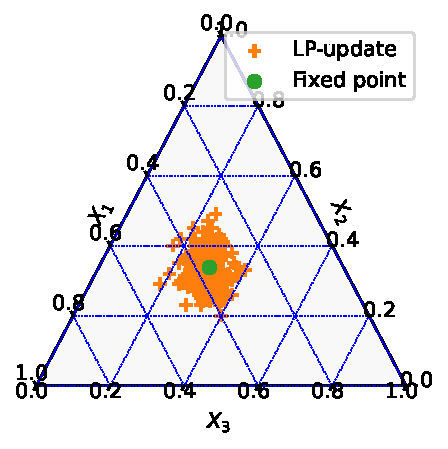
\includegraphics[width=.25\linewidth]{counter-example-GGY2_LP-update.pdf}
        &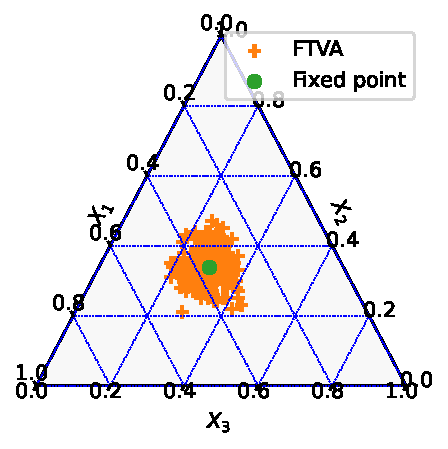
\includegraphics[width=.25\linewidth]{counter-example-GGY2_FTVA.pdf}
        &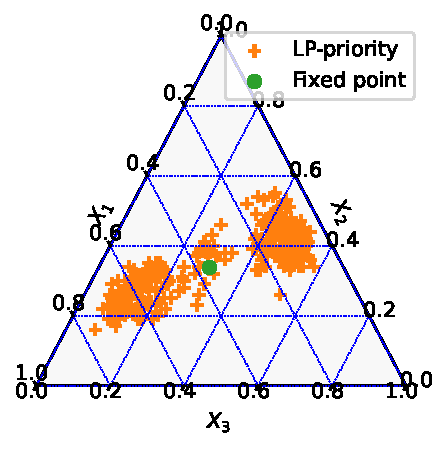
\includegraphics[width=.25\linewidth]{counter-example-GGY2_LP-priority.pdf}
        &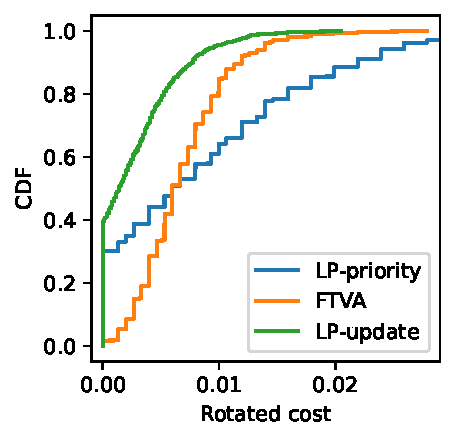
\includegraphics[width=.25\linewidth]{counter-example-GGY2_CDF_rotated_cost_LP-update.pdf}\\
        (a) LP-update
        &(b) FTVA
        &(c) LP-priority        
        &(d) CDF of rotated cost
    \end{tabular}

    \caption{Example~2 from Gast et al. 22. Simulation for $N=100$.}

    \label{fig:example-chen}
\end{figure}

\paragraph{Influence of parameters} Figure~\ref{fig:gain_function_parameters}, studies the influence of different parameters on the performance of LP-update. In each case, we generated $20$ examples and plot the average ``normalized'' performance among these examples. %By ``normalized'', we mean that for each example, we divide the performance of the policy by the value of the LP problem \eqref{EQ::VOPTDYN-Tinf}. The first plot~\ref{fig:gain_function_parameters}(a) shows that the influence of the parameter $\tau$ is marginal (the curves are not distinguishable for $\tau\in\{3,5,10\}$).  In the second plot \ref{fig:gain_function_parameters}(b), we observe that the sub-optimality gap of LP-update does not seem to depend much on the state space size whereas the one of FTVA does: FTVA performs worse when $|\sspace|$ is large probably because there are fewer synchronized arms. In the last plot \ref{fig:gain_function_parameters}(c), we study the performance as a function of the budget parameter, $\alpha$.
%%%%%%%%%
``normalized'' here means we divide the performance of the policy by the value of the LP problem \eqref{EQ::VOPTDYN-Tinf}. The first plot~\ref{fig:gain_function_parameters}(a) shows that the influence of the parameter $\tau$ is marginal (the curves are not distinguishable for $\tau\in\{3,5,10\}$).  Plot \ref{fig:gain_function_parameters}(b) indicates that the sub-optimality gap of LP-update is not too sensitive to the state space size unlike FTVA which degrades when $|\sspace|$ is large probably because there are fewer synchronized arms. The last plot \ref{fig:gain_function_parameters}(c) studies the performance as a function of the budget parameter, $\alpha$. %\redtext{ as before, the sub-optimality gap} 
\begin{figure}[t]
    \centering
    \begin{tabular}{@{}c@{}c@{}c@{}}
        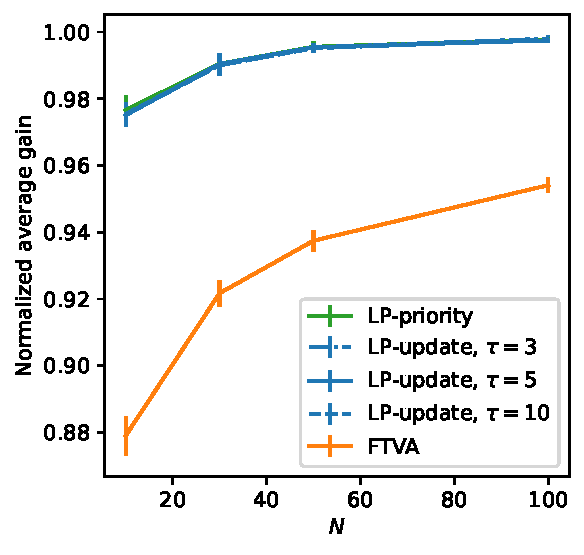
\includegraphics[width=0.33\linewidth]{gain_various_tau.pdf}
        &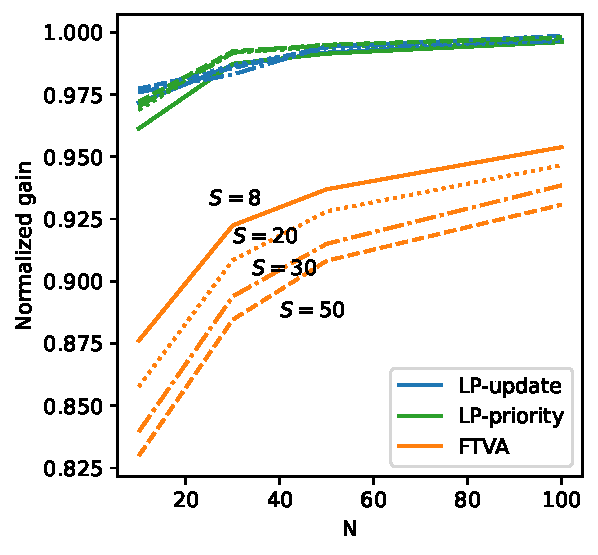
\includegraphics[width=0.33\linewidth]{gain_various_S.pdf}
        &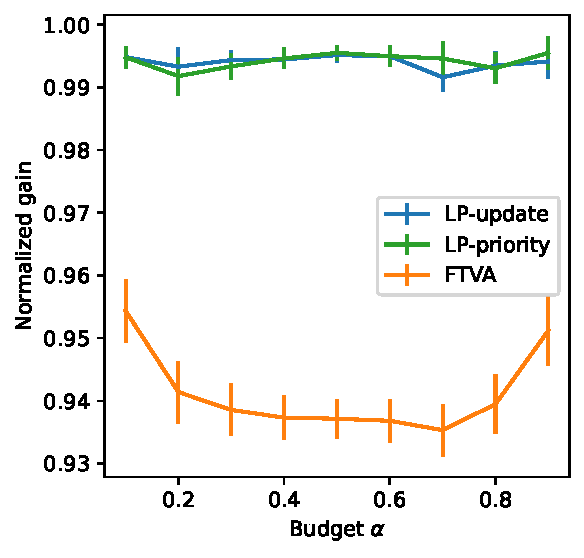
\includegraphics[width=0.33\linewidth]{gain_various_alpha.pdf}\\
        (a) For various $\tau$.
        &(b) For various $S$.
        &(c) For various $\alpha$ ($N=50$).
    \end{tabular}

    \caption{Comparison of the gains as a function of some parameters.}
    \label{fig:gain_function_parameters}
\end{figure}